\chapter{Chengdu, Emeishan et Leshan}
\section*{8 octobre 2015}
Chengdu est une immense ville de plusieurs millions d'habitants \newline
 Place centrale avec une statue de Mao \newline
 \newline
\centerline{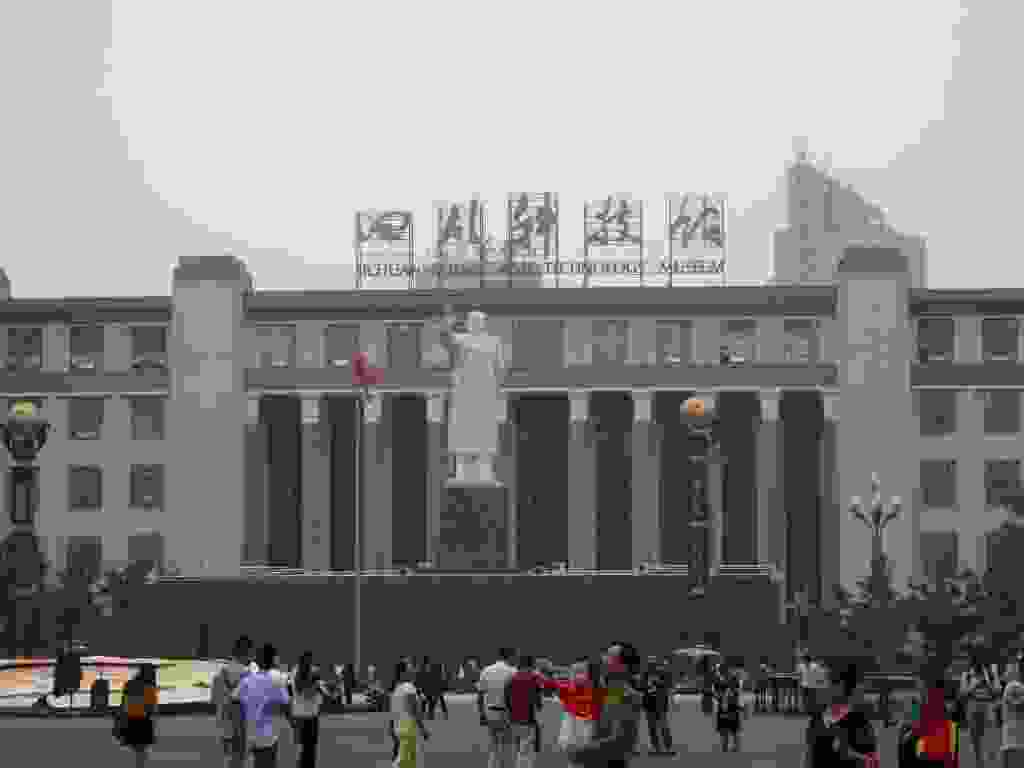
\includegraphics[height=90mm]{../wp-content/uploads/2015/09/wpid-p9227084-1024x768.jpg} } 
 \newline
 \newline
\centerline{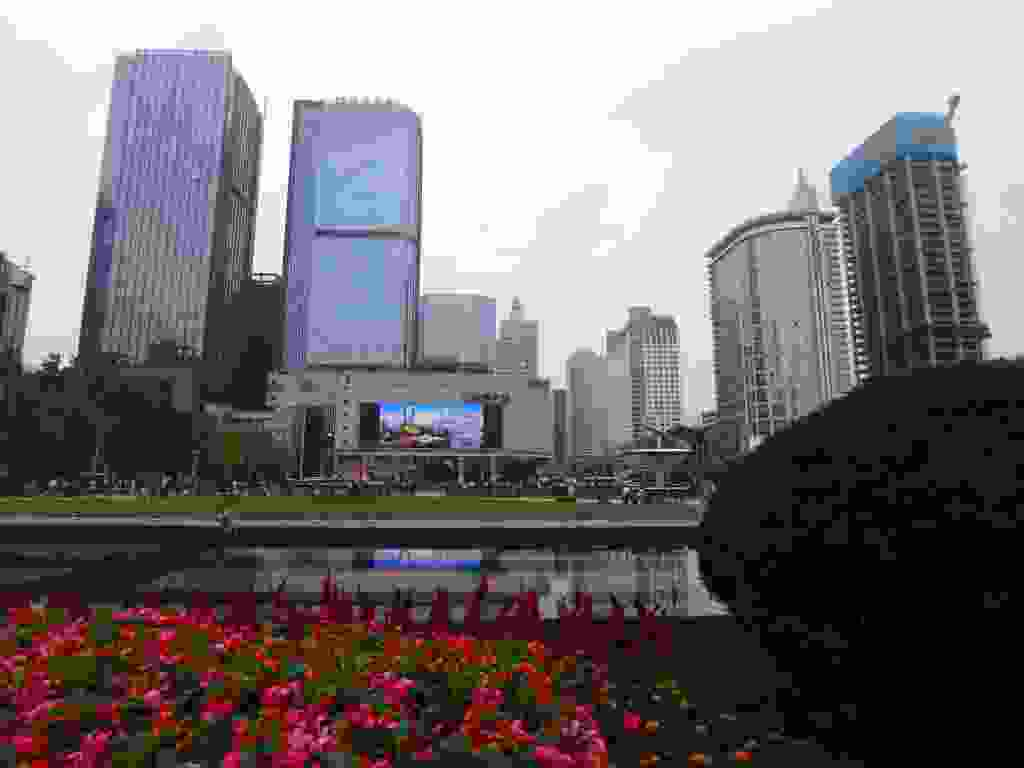
\includegraphics[height=90mm]{../wp-content/uploads/2015/09/wpid-p9227086-1024x768.jpg} } 
 \newline
 People's Park, toujours des activités variées \newline
 \newline
\centerline{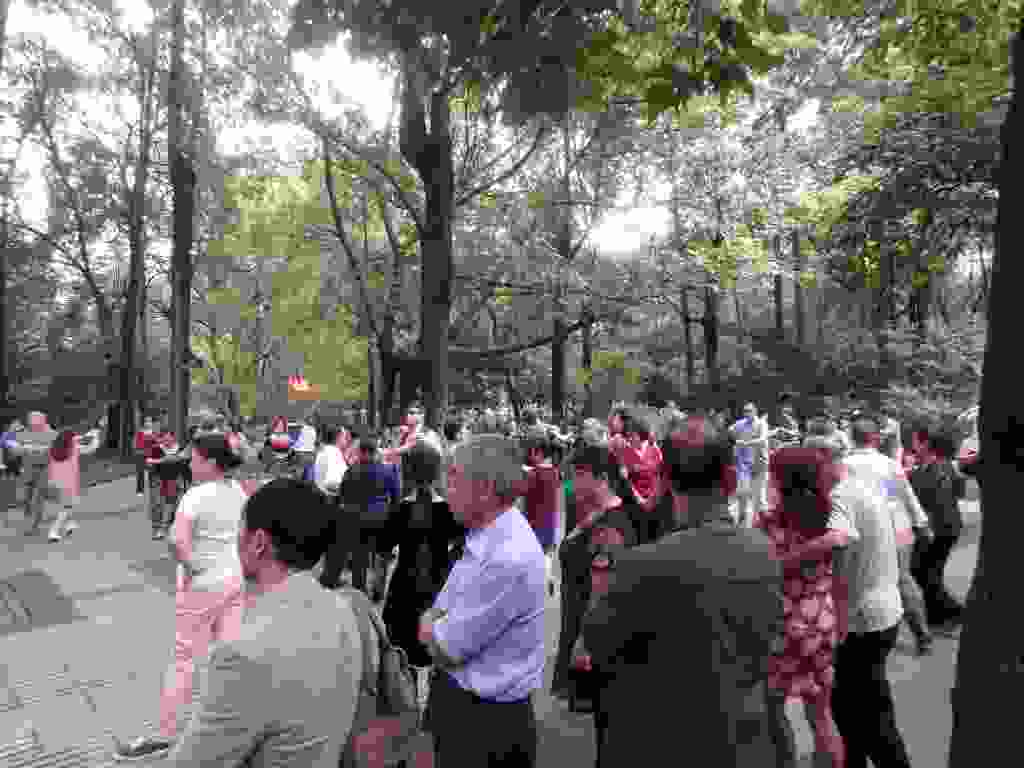
\includegraphics[height=90mm]{../wp-content/uploads/2015/09/wpid-p9227076-1024x768.jpg} } 
 \newline
 \newline
\centerline{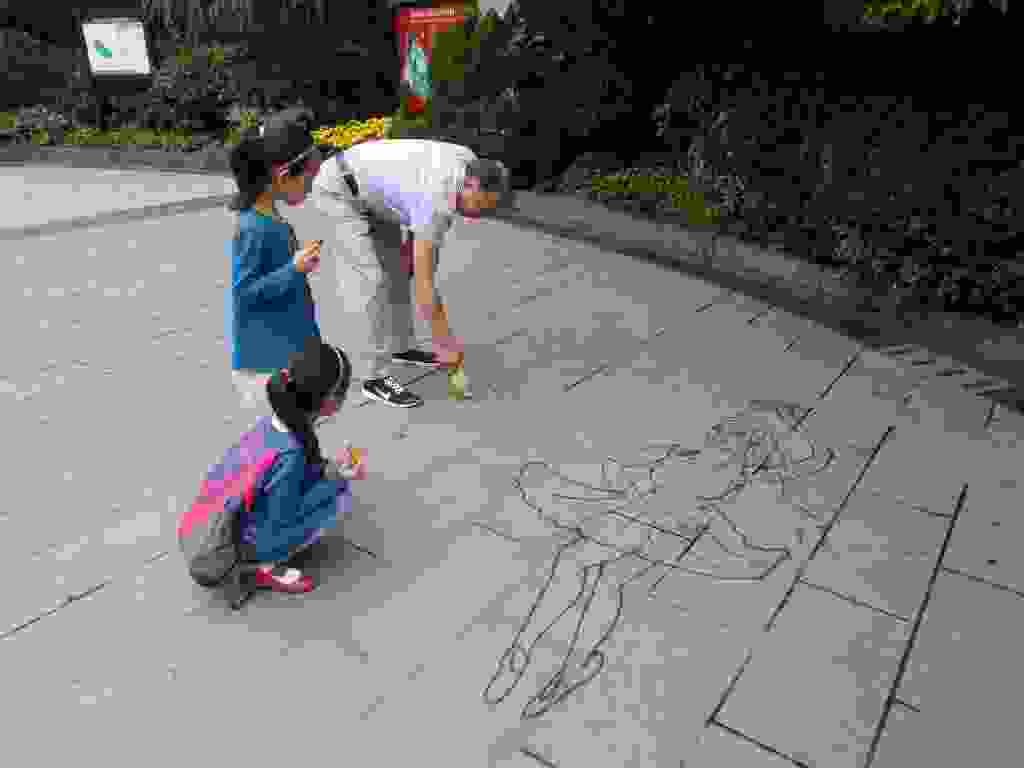
\includegraphics[height=90mm]{../wp-content/uploads/2015/09/wpid-p9227083-1024x768.jpg} } 
 \newline
 \newline
\centerline{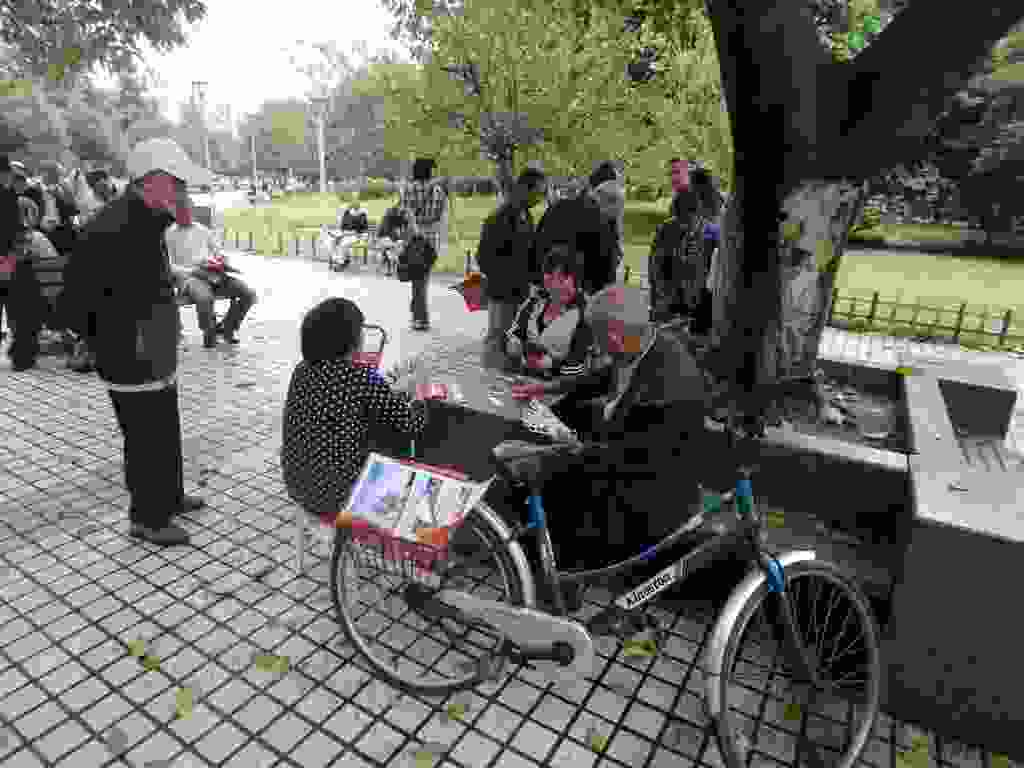
\includegraphics[height=90mm]{../wp-content/uploads/2015/10/wpid-p9270005-1024x768.jpg} } 
 \newline
 Dans une allée, des parents déposent des annonces pour marier leur fille, une seule était en anglais : \newline
 \newline
\centerline{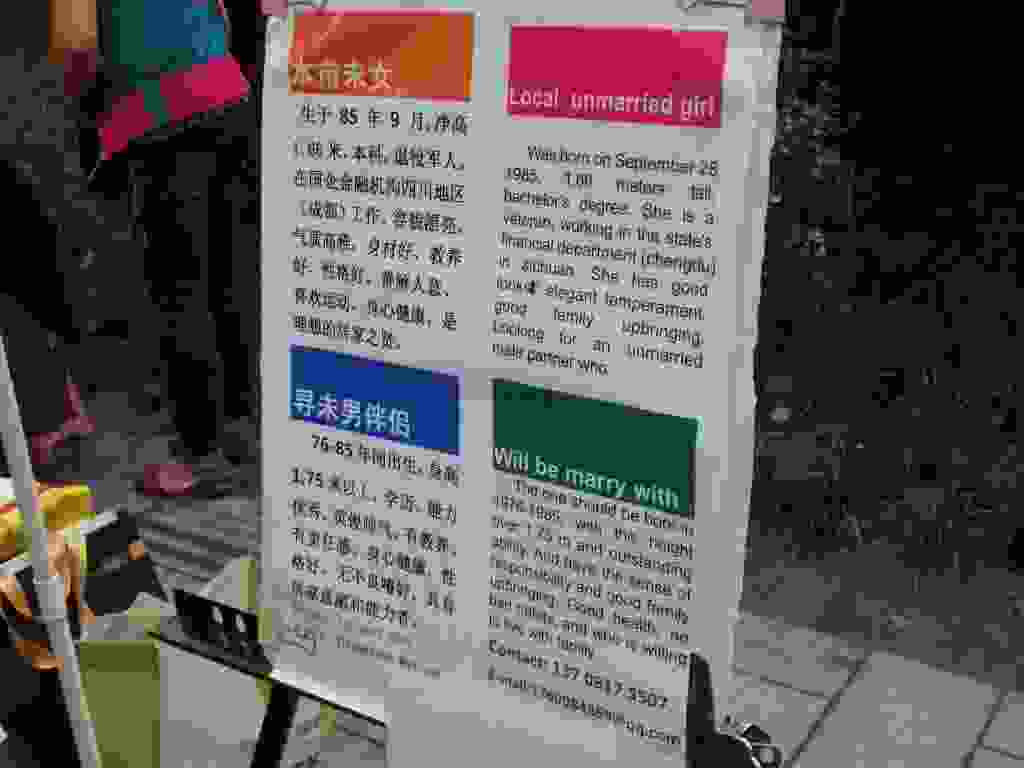
\includegraphics[height=90mm]{../wp-content/uploads/2015/09/wpid-p9227079-1024x768.jpg} } 
 \newline
 Monastère bouddhiste de Wenshu \newline
 \newline
\centerline{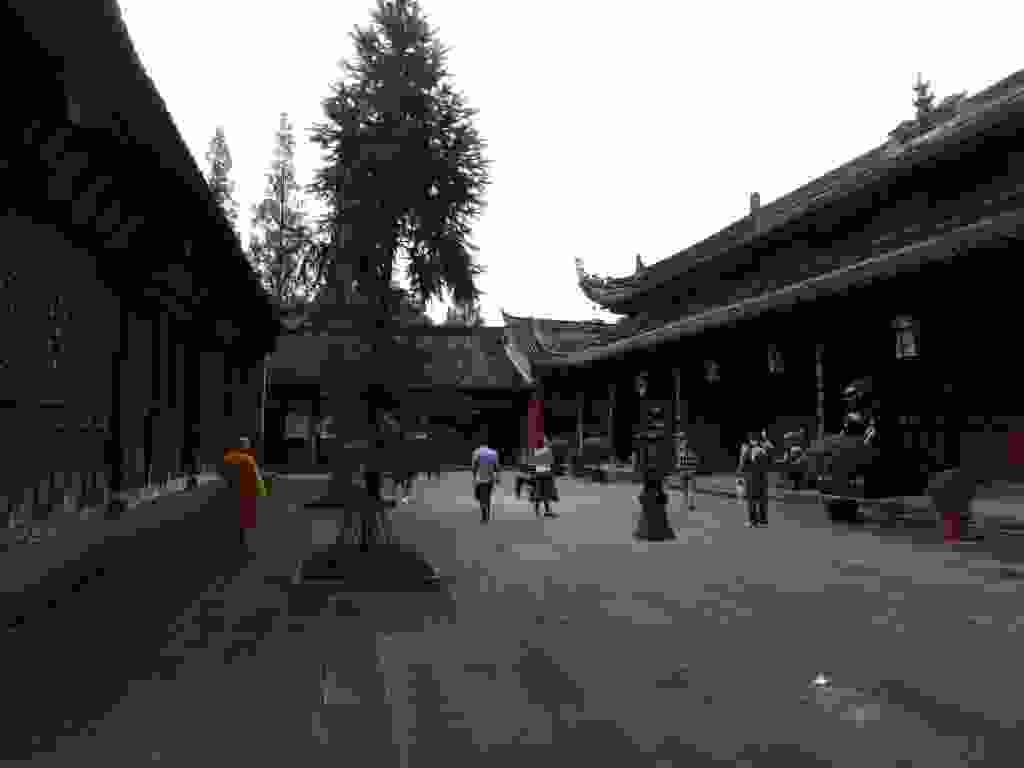
\includegraphics[height=90mm]{../wp-content/uploads/2015/10/wpid-p92270651-1024x768.jpg} } 
 \newline
 \newline
\centerline{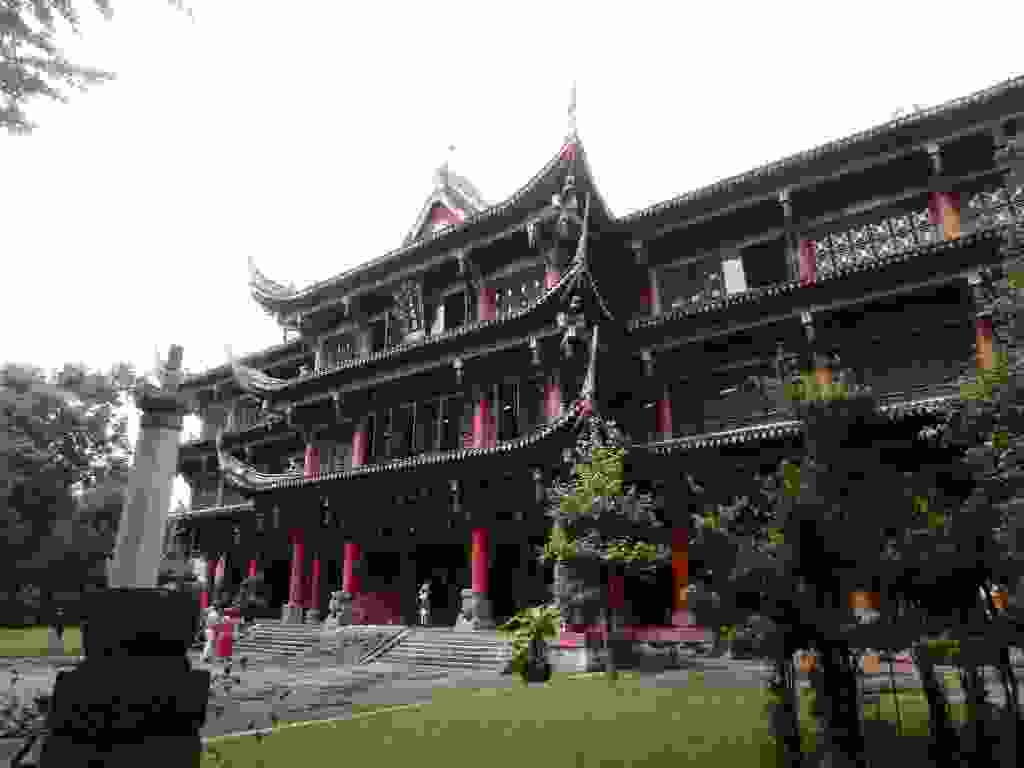
\includegraphics[height=90mm]{../wp-content/uploads/2015/09/wpid-p9227068-1024x768.jpg} } 
 \newline
 \newline
\centerline{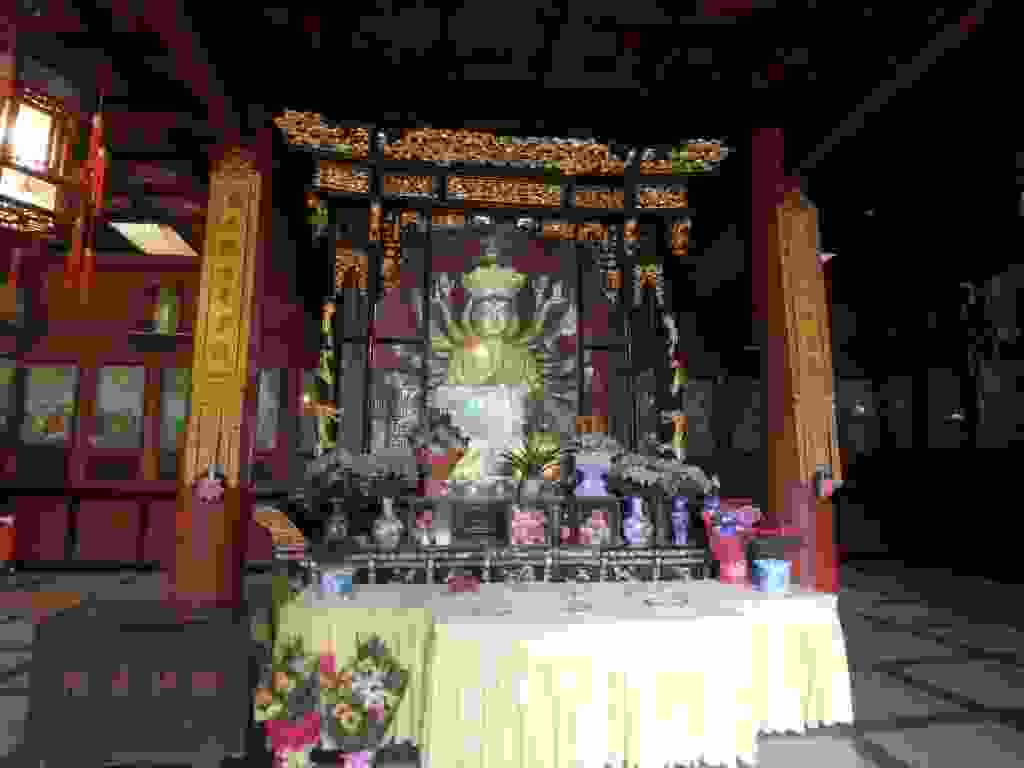
\includegraphics[height=90mm]{../wp-content/uploads/2015/09/wpid-p9227066-1024x768.jpg} } 
 \newline
 Dans l'hostel où je suis à Chengdu, je rencontre Fred et Brigitte, cyclistes suisses qui roulent depuis 1 an et demi, ils ont traversé toute l'Europe puis l'Asie centrale avant d'arriver en Chine. Ils voyagent depuis 1 semaine avec Jet, chinois. \newline
 \newline
\centerline{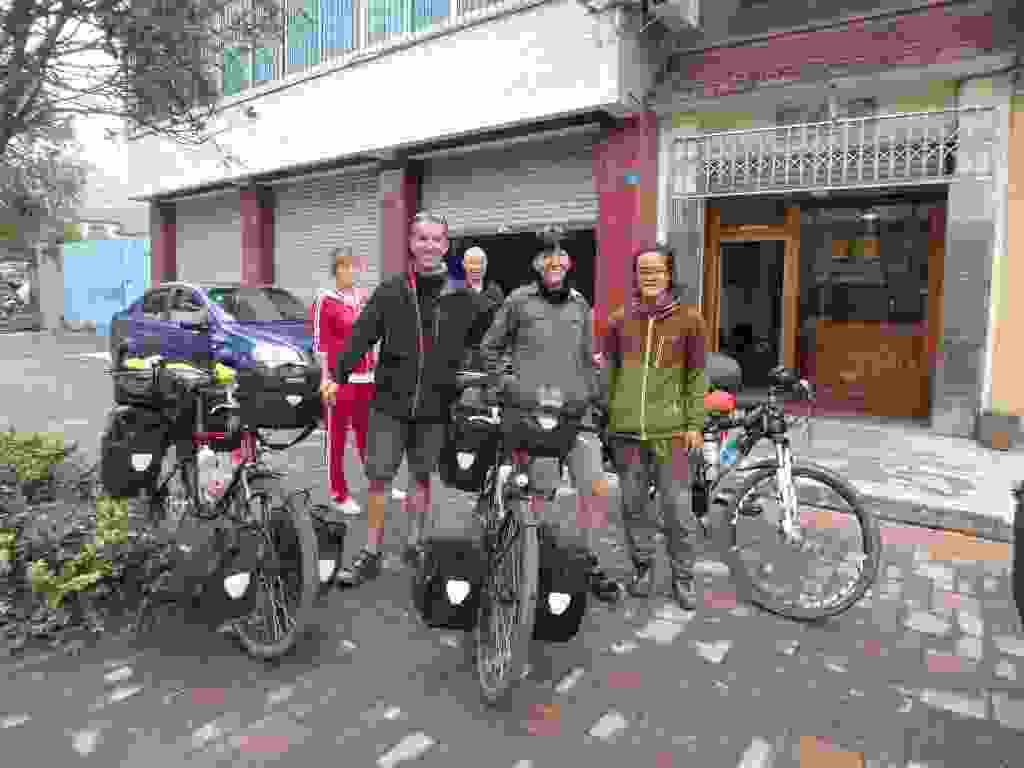
\includegraphics[height=90mm]{../wp-content/uploads/2015/09/wpid-p92070201-1024x768.jpg} } 
 \newline
 Comme ils vont vers le Sud, je me joins à eux pour quelques jours. \newline
 \newline
\centerline{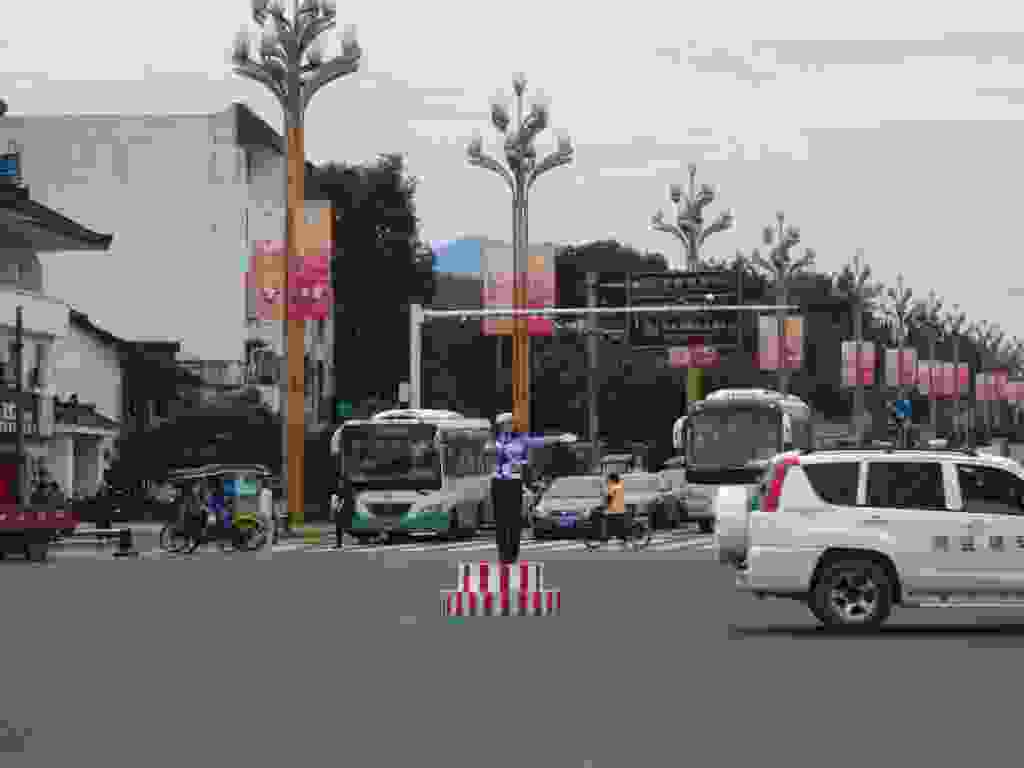
\includegraphics[height=90mm]{../wp-content/uploads/2015/10/wpid-p9257115-1024x768.jpg} } 
 \newline
 Sortie de la ville, on n'est pas perdu pour faire les courses \newline
 \newline
\centerline{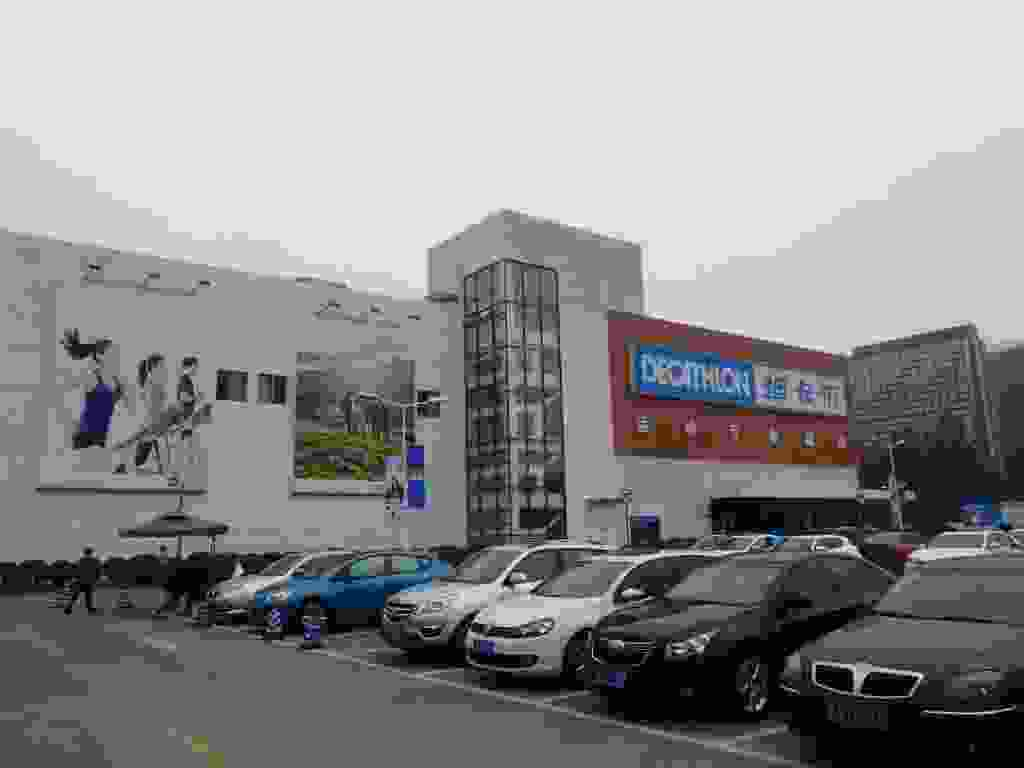
\includegraphics[height=90mm]{../wp-content/uploads/2015/09/wpid-p9237090-1024x768.jpg} } 
 \newline
 \newline
\centerline{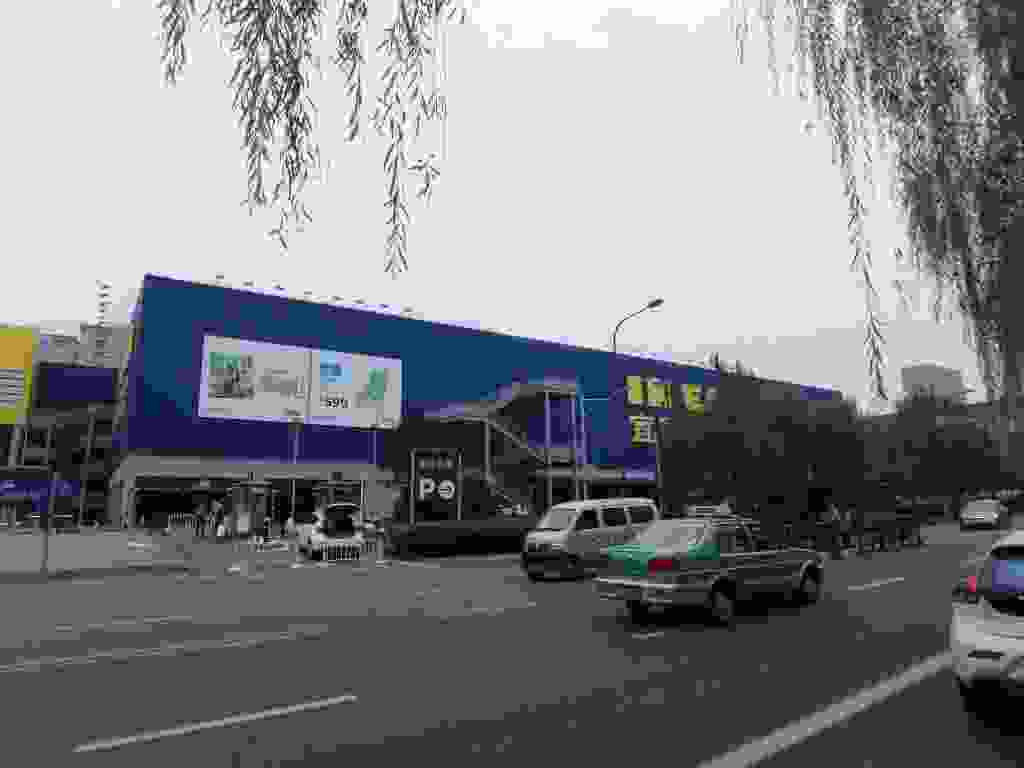
\includegraphics[height=90mm]{../wp-content/uploads/2015/10/wpid-p9237091-1024x768.jpg} } 
 \newline
 Ce bâtiment est sensé être le plus gros du monde \newline
 \newline
\centerline{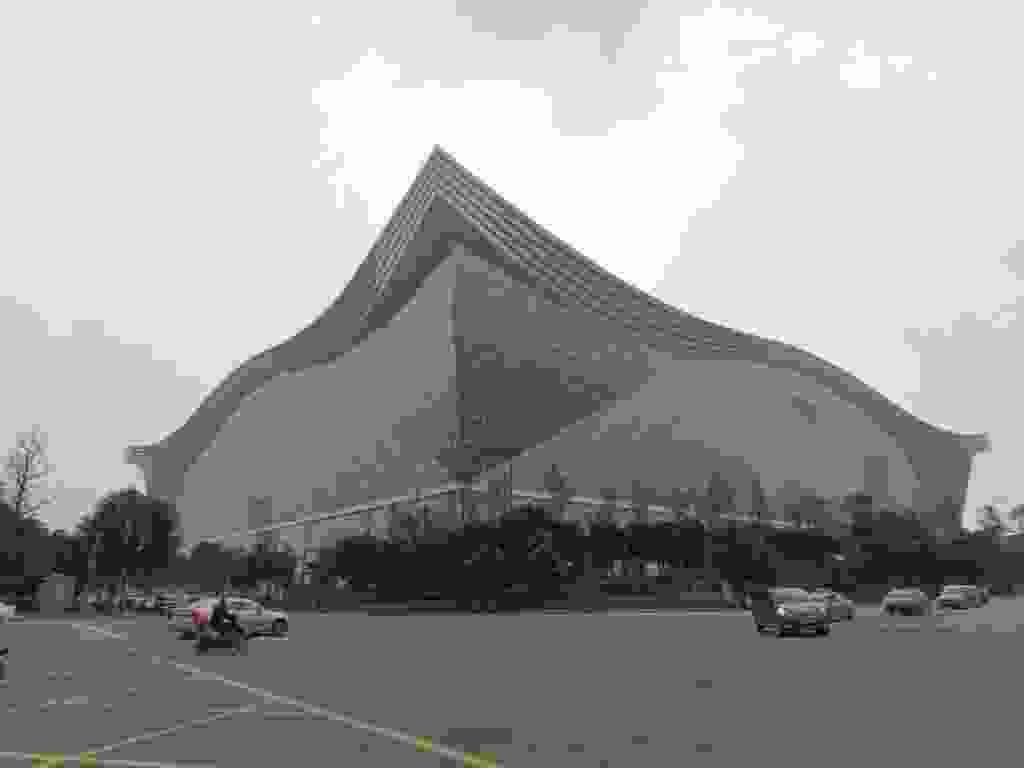
\includegraphics[height=90mm]{../wp-content/uploads/2015/09/wpid-p9237095-1024x768.jpg} } 
 \newline
 Bivouacs à 3 tentes \newline
 \newline
\centerline{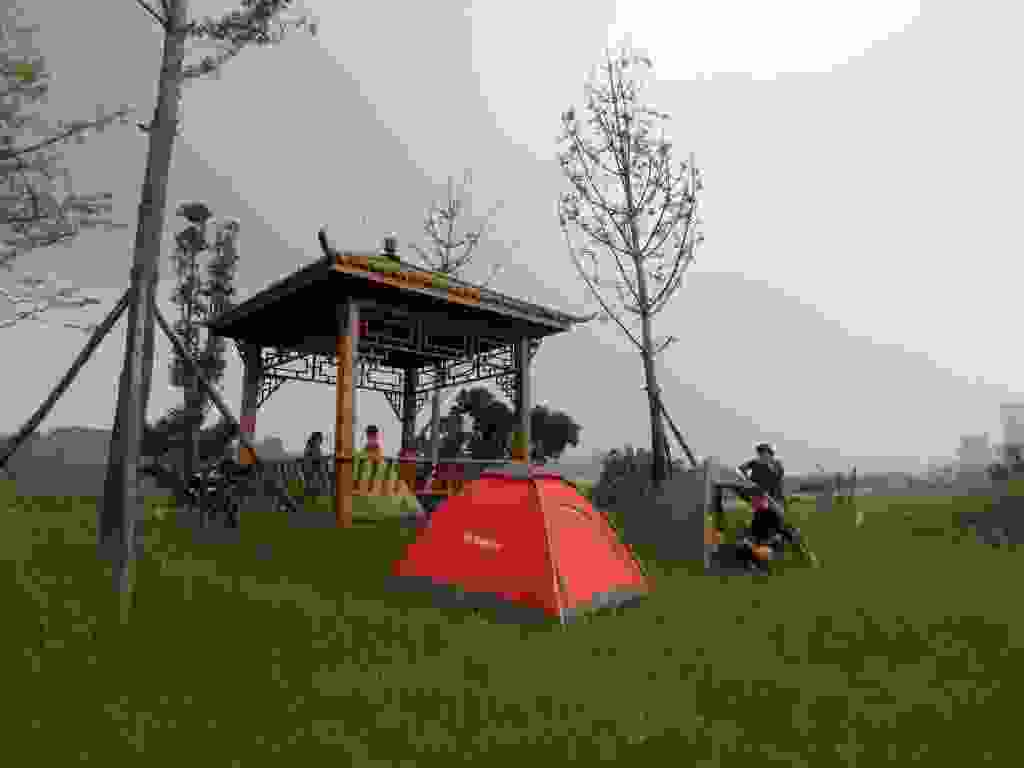
\includegraphics[height=90mm]{../wp-content/uploads/2015/09/wpid-p9237104-1024x768.jpg} } 
 \newline
 Visite de Huanglongxi, petit village touristique \newline
 \newline
\centerline{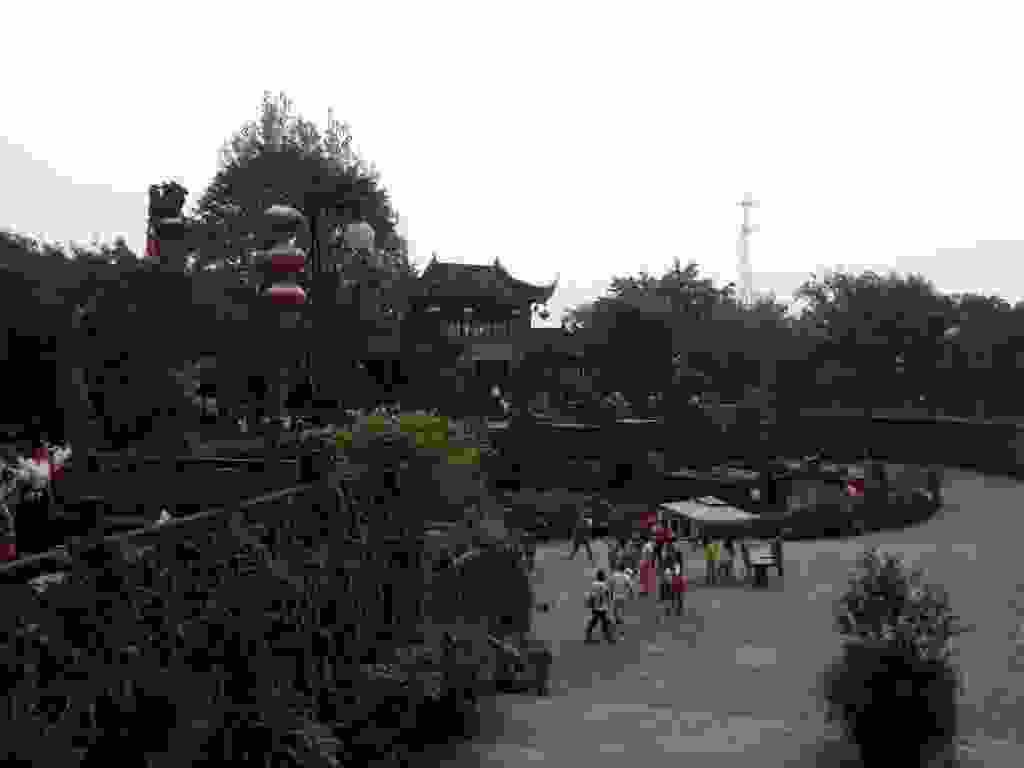
\includegraphics[height=90mm]{../wp-content/uploads/2015/09/wpid-p9237098-1024x768.jpg} } 
 \newline
 \newline
\centerline{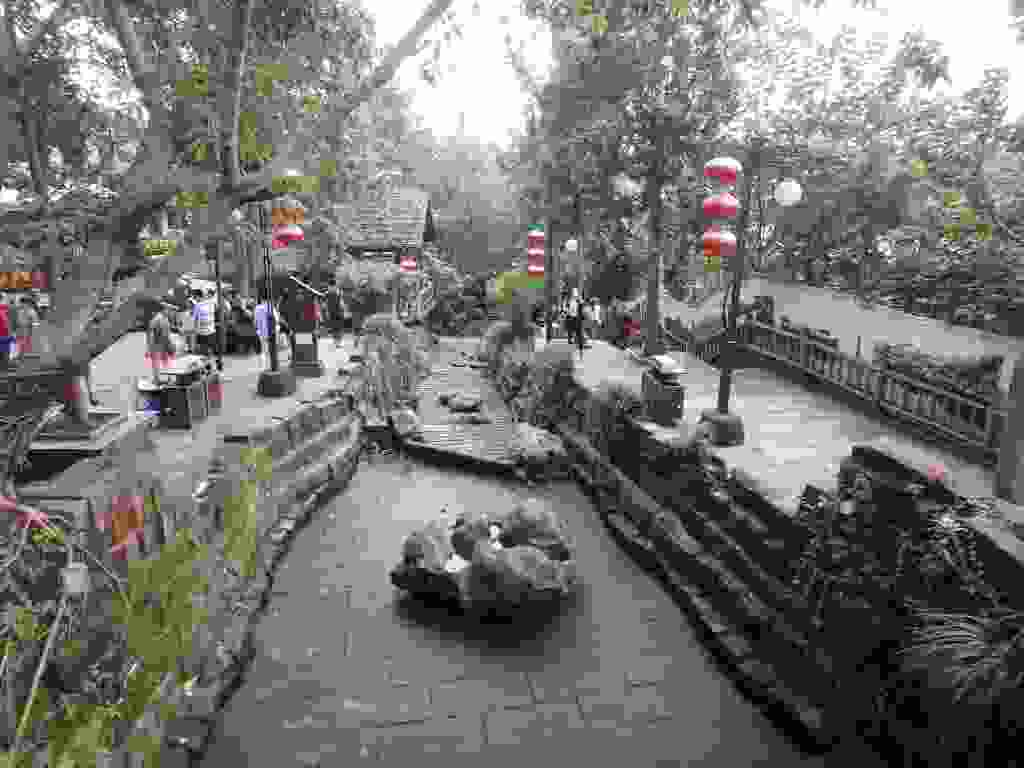
\includegraphics[height=90mm]{../wp-content/uploads/2015/09/wpid-p9237099-1024x768.jpg} } 
 \newline
 Nous allons voir Emeishan, montagne sacrée du bouddhisme. Montée en bus au sommet à plus de 3000m \newline
 \newline
\centerline{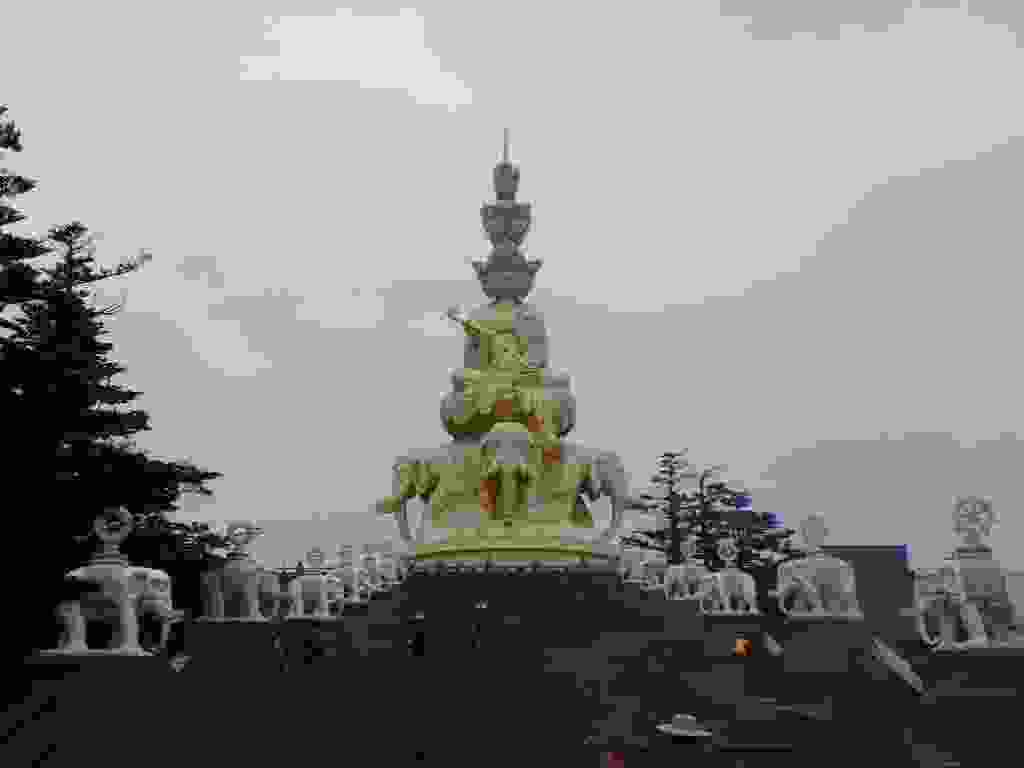
\includegraphics[height=90mm]{../wp-content/uploads/2015/09/wpid-p9257125-1024x768.jpg} } 
 \newline
 \newline
\centerline{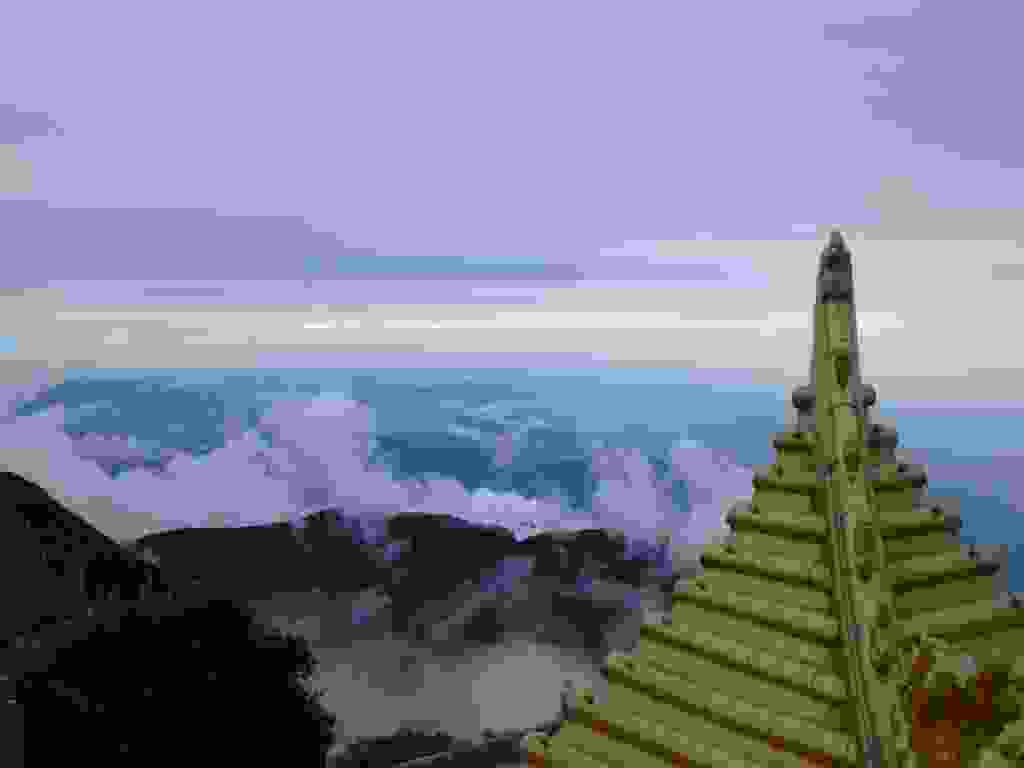
\includegraphics[height=90mm]{../wp-content/uploads/2015/09/wpid-p9257131-1024x768.jpg} } 
 \newline
 \newline
\centerline{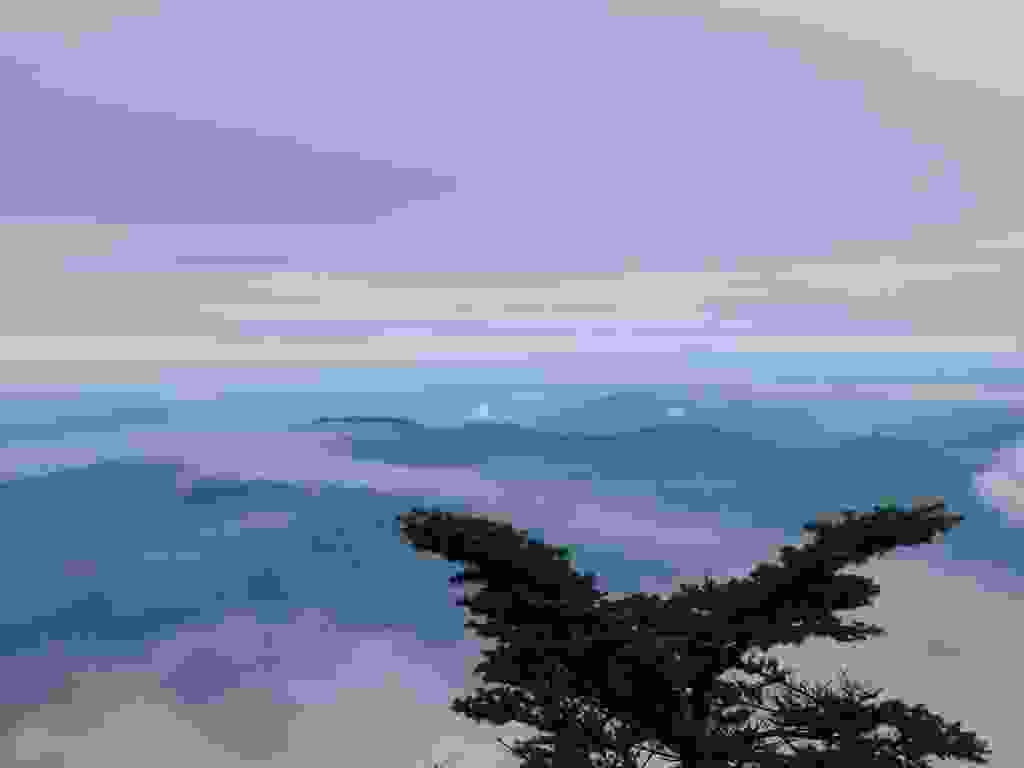
\includegraphics[height=90mm]{../wp-content/uploads/2015/09/wpid-p9257133-1024x768.jpg} } 
 \newline
 Descente à pied jusqu'en bas, que des marches : après ça impossible de prendre un escalier pendant 3 jours \newline
 \newline
\centerline{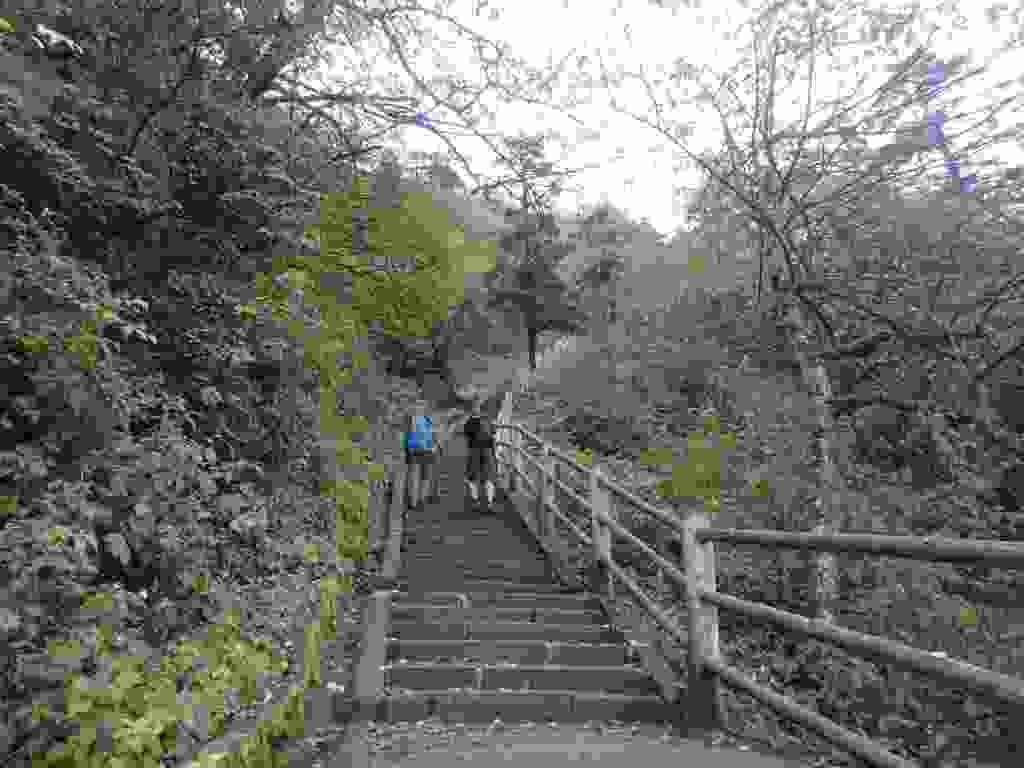
\includegraphics[height=90mm]{../wp-content/uploads/2015/09/wpid-p9257123-1024x768.jpg} } 
 \newline
 Les singes sont habitués à voler la nourriture \newline
 \newline
\centerline{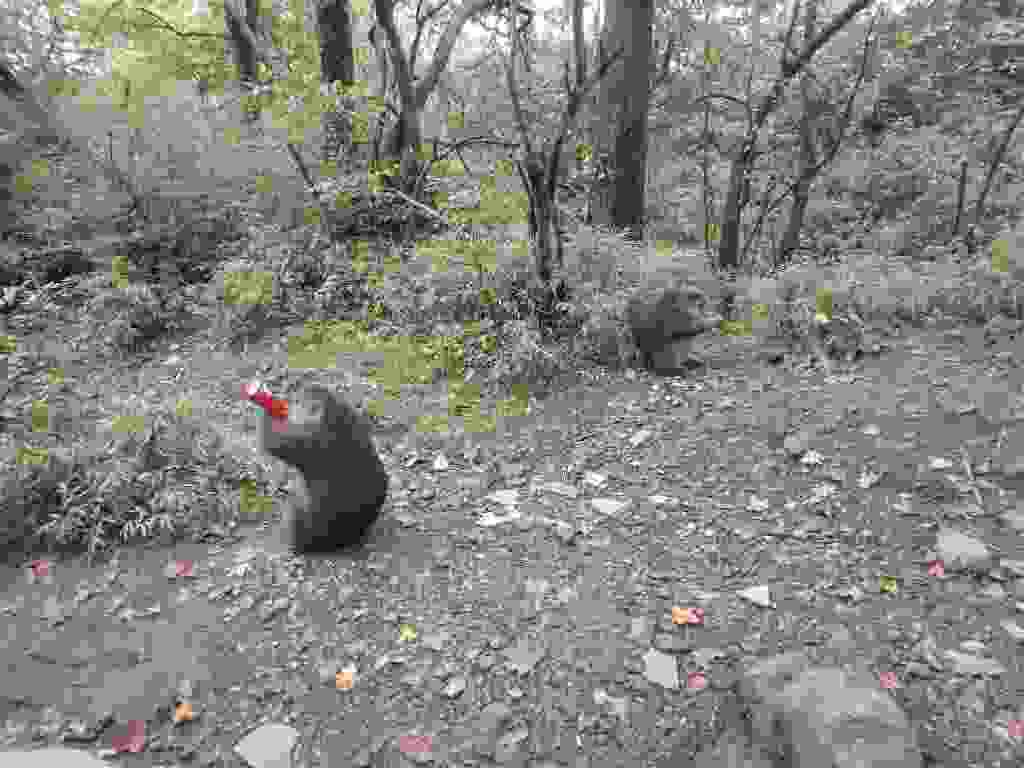
\includegraphics[height=90mm]{../wp-content/uploads/2015/09/wpid-p9257118-1024x768.jpg} } 
 \newline
 On croise régulièrement des temples sur le chemin \newline
 \newline
\centerline{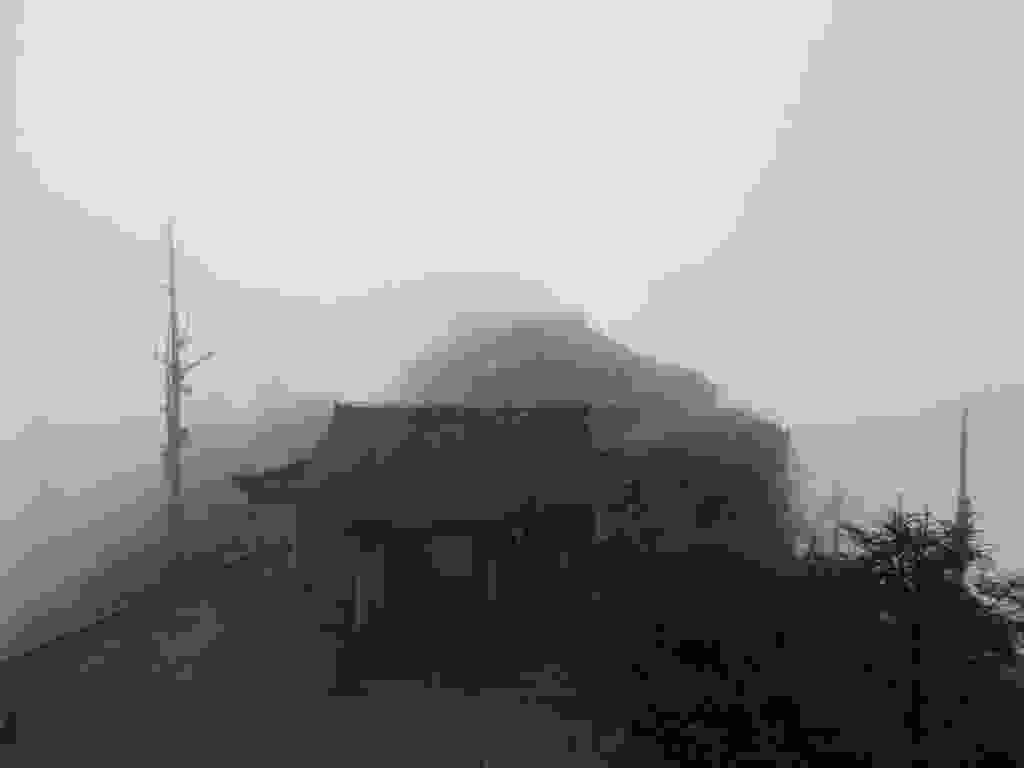
\includegraphics[height=90mm]{../wp-content/uploads/2015/09/wpid-p9267140-1024x768.jpg} } 
 \newline
 \newline
\centerline{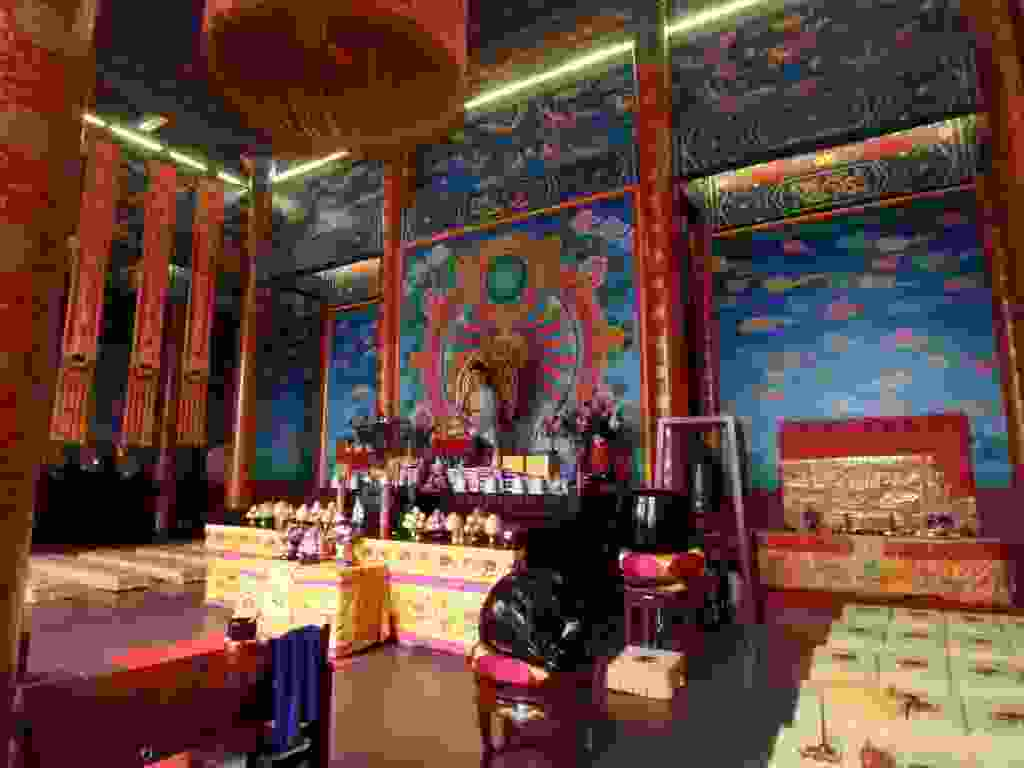
\includegraphics[height=90mm]{../wp-content/uploads/2015/09/wpid-p9267139-1024x768.jpg} } 
 \newline
 \newline
\centerline{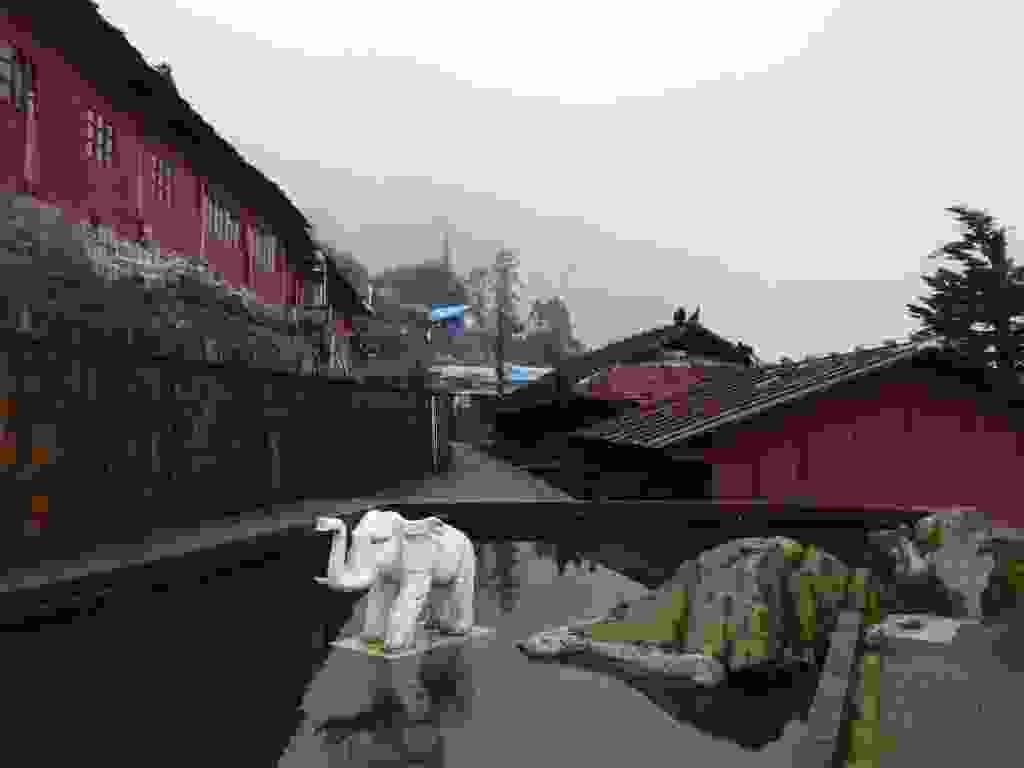
\includegraphics[height=90mm]{../wp-content/uploads/2015/09/wpid-p9267144-1024x768.jpg} } 
 \newline
 \newline
\centerline{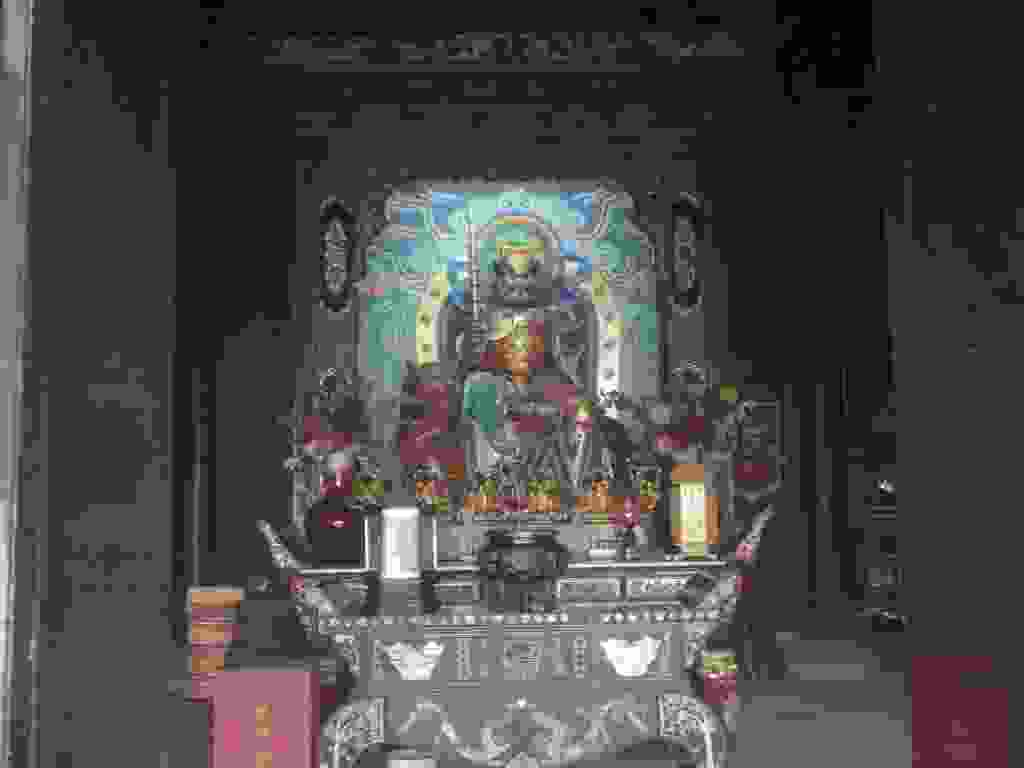
\includegraphics[height=90mm]{../wp-content/uploads/2015/09/wpid-p9267149-1024x768.jpg} } 
 \newline
 \newline
\centerline{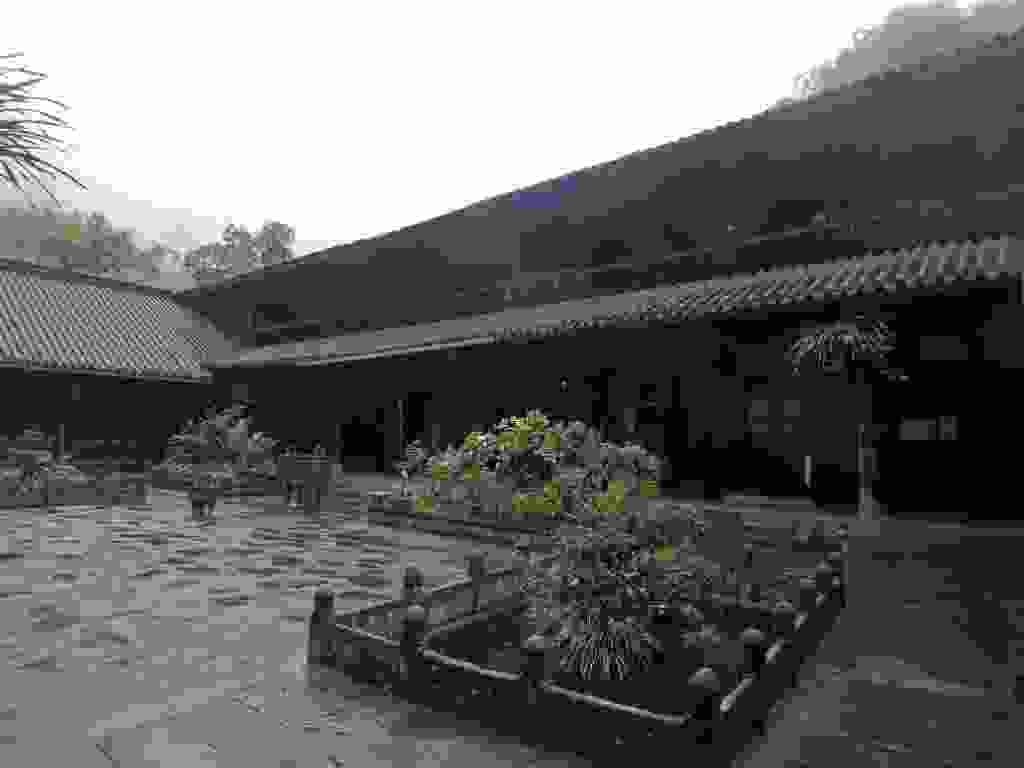
\includegraphics[height=90mm]{../wp-content/uploads/2015/09/wpid-p9267154-1024x768.jpg} } 
 \newline
 \newline
\centerline{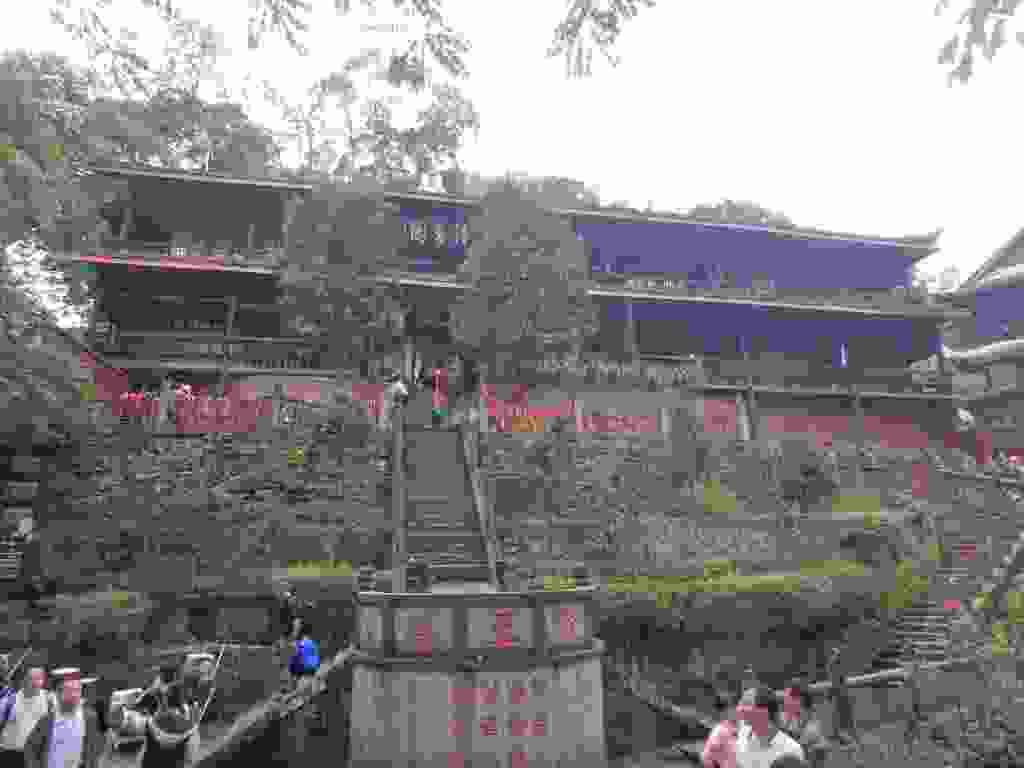
\includegraphics[height=90mm]{../wp-content/uploads/2015/09/wpid-p9267161-1024x768.jpg} } 
 \newline
 La route continue vers Leshan où je dois renouveler mon visa pour 1 mois de plus. L'occasion d'aller voir le Grand Bouddha de Leshan. \newline
 On passe d'abord par un temple \newline
 \newline
\centerline{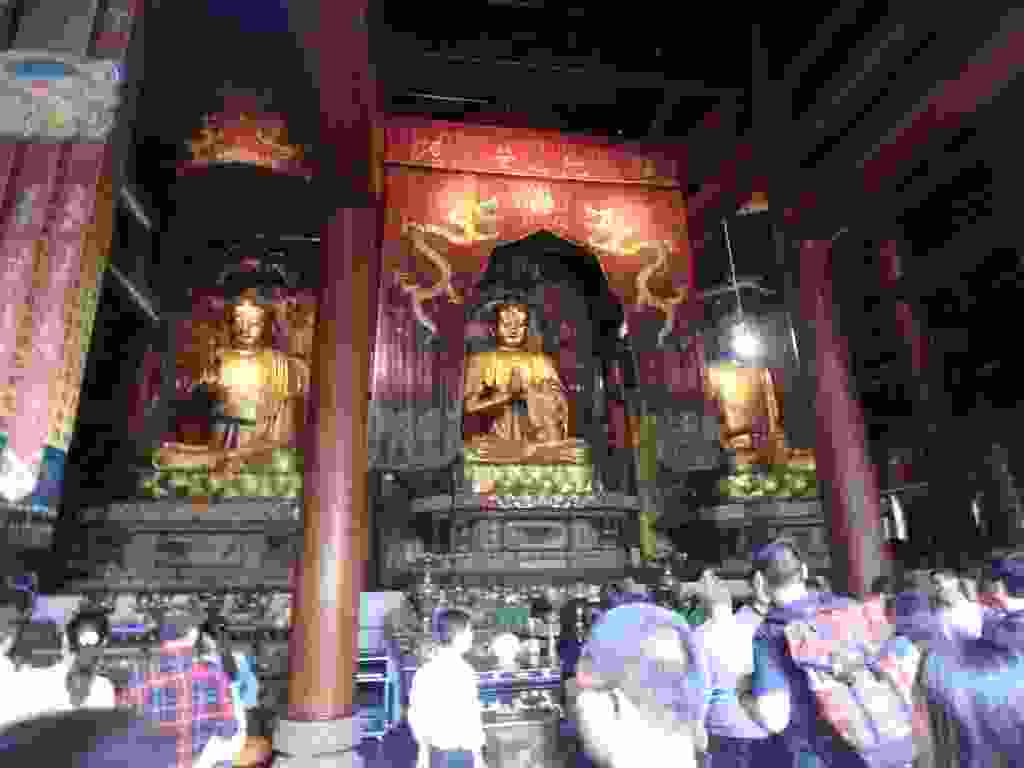
\includegraphics[height=90mm]{../wp-content/uploads/2015/09/wpid-p9280013-1024x768.jpg} } 
 \newline
 \newline
\centerline{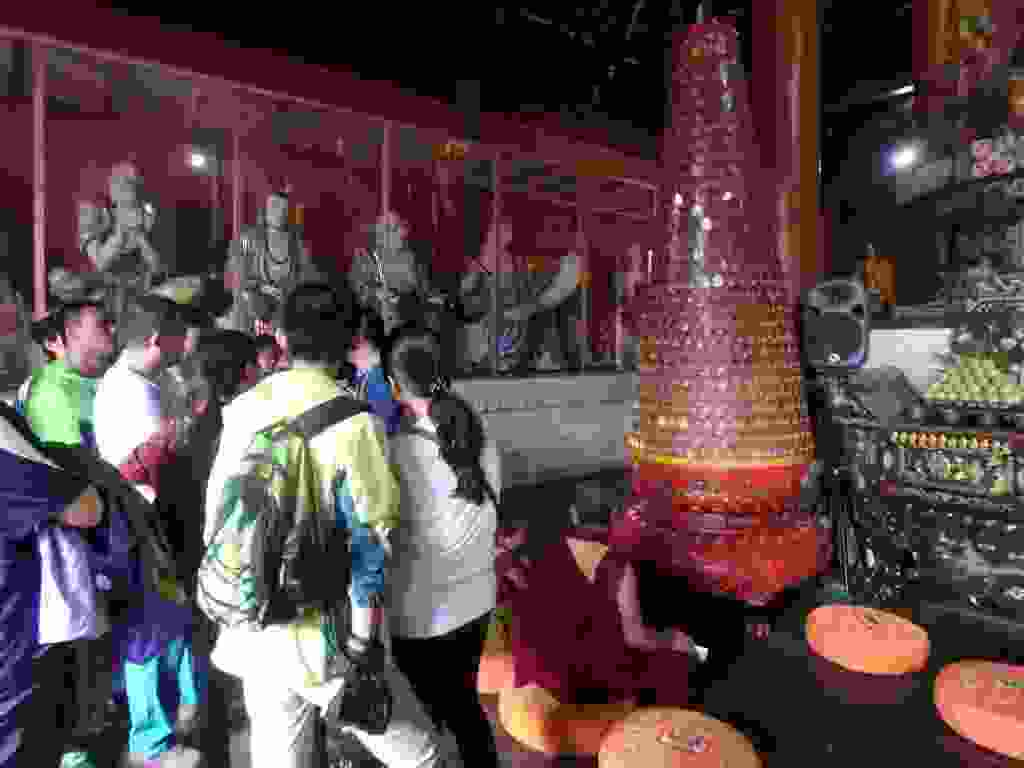
\includegraphics[height=90mm]{../wp-content/uploads/2015/09/wpid-p9280014-1024x768.jpg} } 
 \newline
 \newline
\centerline{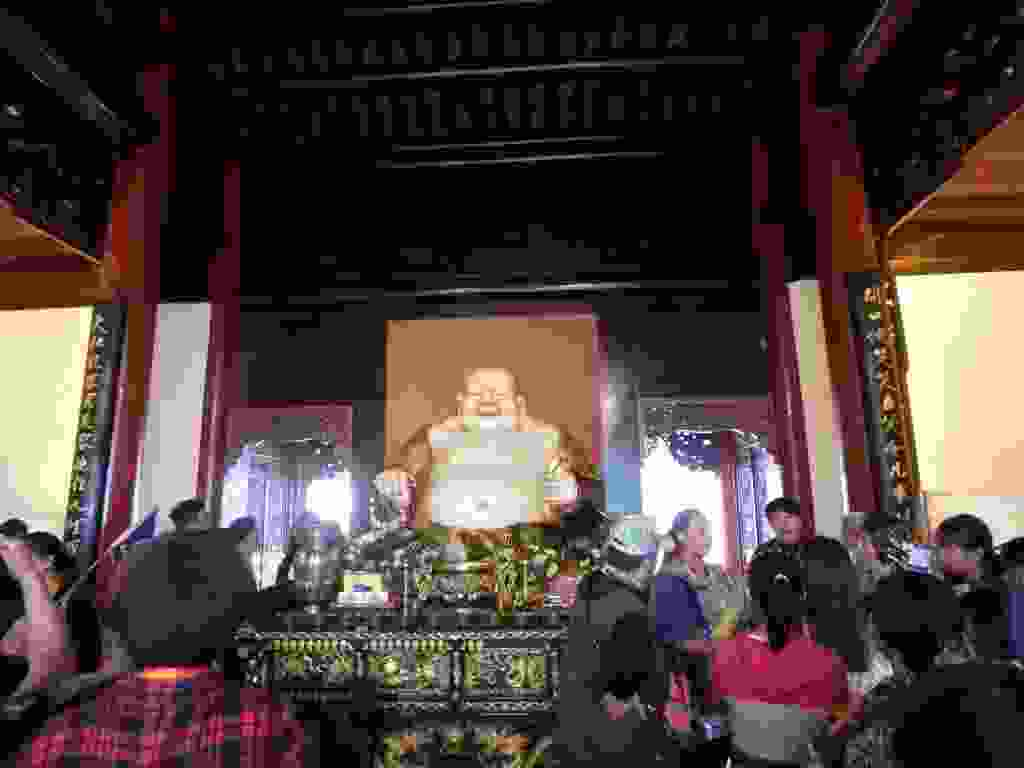
\includegraphics[height=90mm]{../wp-content/uploads/2015/09/wpid-p9280015-1024x768.jpg} } 
 \newline
 Avant la descente vers le bouddha : 71m de haut \newline
 \newline
\centerline{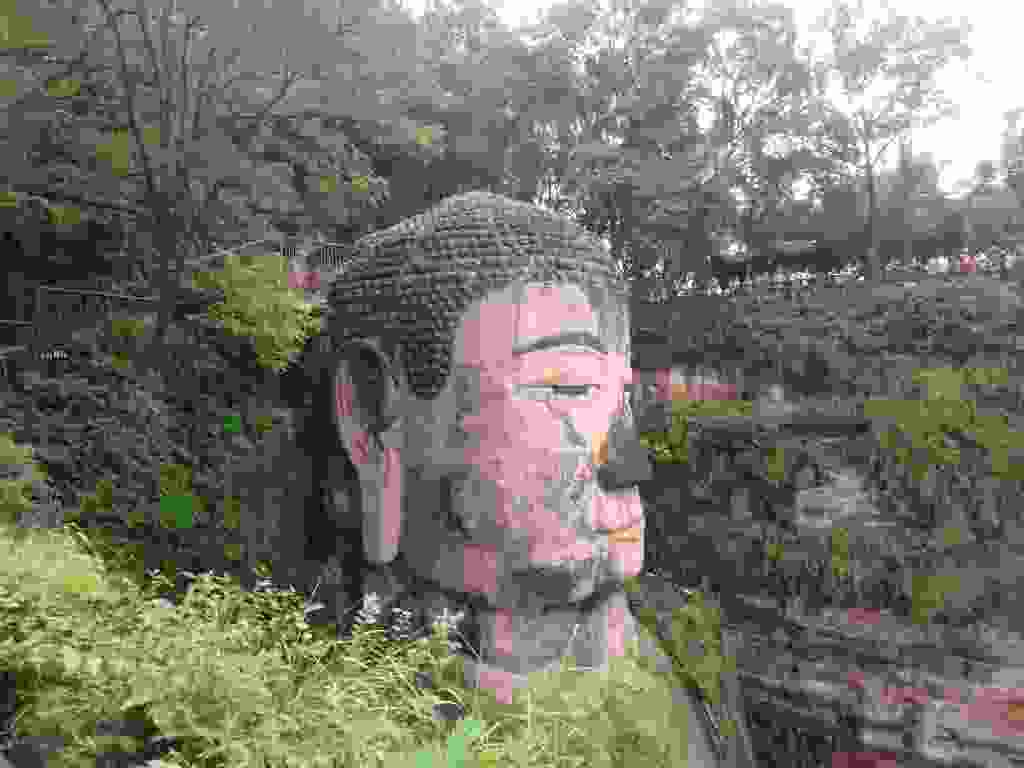
\includegraphics[height=90mm]{../wp-content/uploads/2015/09/wpid-p9280016-1024x768.jpg} } 
 \newline
 \newline
\centerline{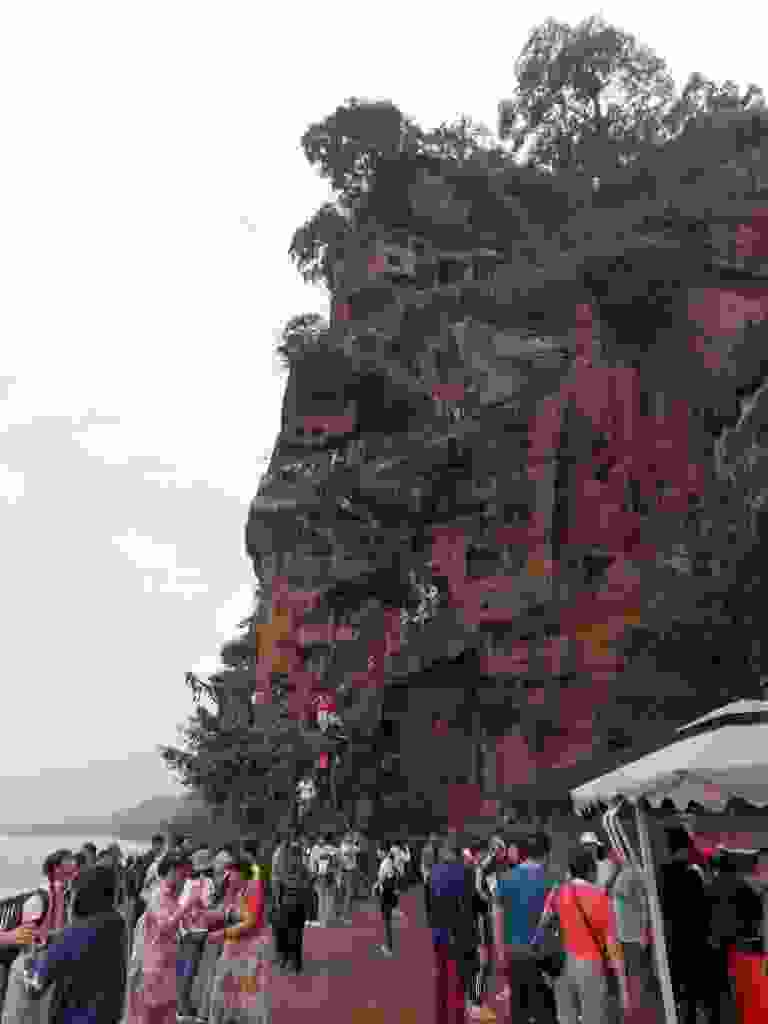
\includegraphics[height=90mm]{../wp-content/uploads/2015/09/wpid-p9280028-e1444295218575-768x1024.jpg} } 
 \newline
 \newline
\centerline{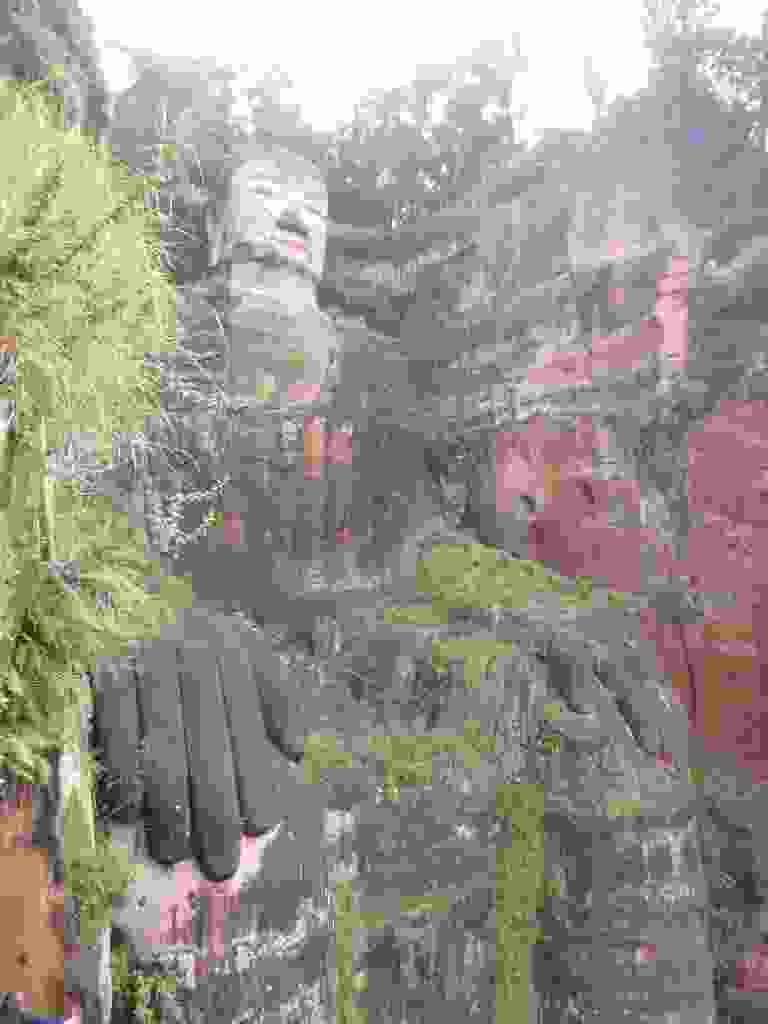
\includegraphics[height=90mm]{../wp-content/uploads/2015/10/wpid-p9280024-e1444295278311-768x1024.jpg} } 
 \newline
 \newline
\centerline{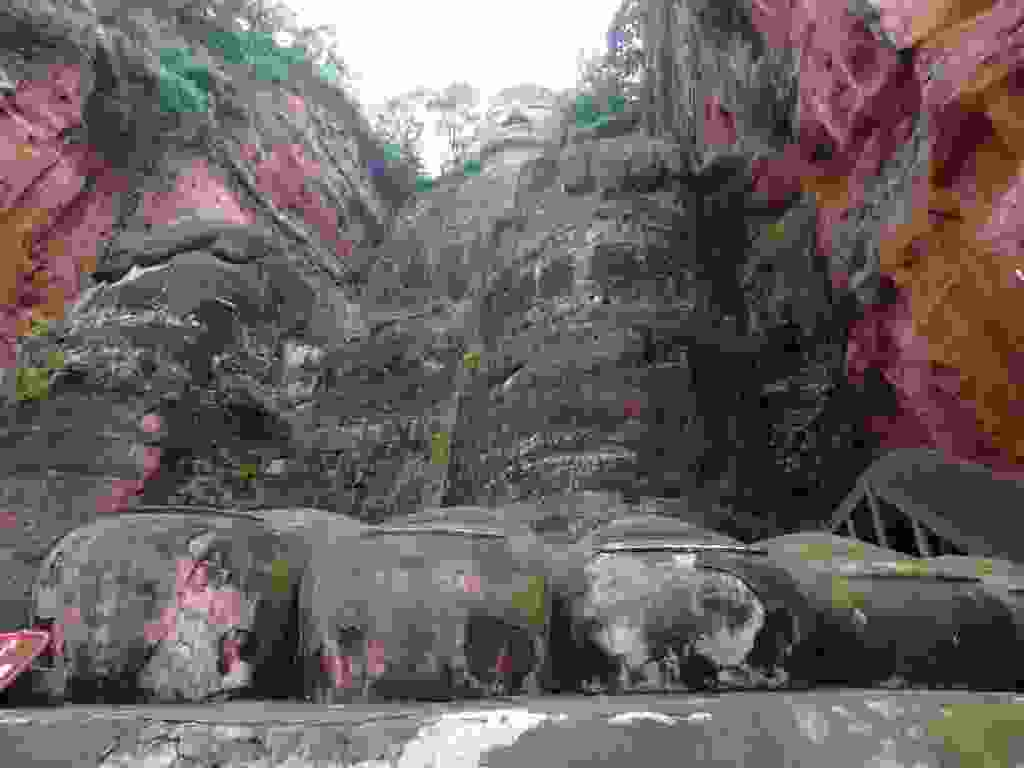
\includegraphics[height=90mm]{../wp-content/uploads/2015/09/wpid-p9280029-1024x768.jpg} } 
 \newline

\newpage
 
